\iffalse
\begin{figure}[htbp] %  figure placement: here, top, bottom, or page
   \centering
   \includegraphics[width=2in]{example.jpg} 
   \caption{example caption}
   \label{fig:example}
\end{figure}
\fi

\documentclass[../main.tex]{subfiles}
\begin{document}

\section{Theory}\label{sec:theory}

\subsection{Franke's function}
Franke's function is a function which is often used to test different regression and interpolation methods. The function has two Gaussian peaks of differing heights, and a smaller dip. It's expression is

\begin{align}
\begin{split}
  f(x,y) &= \frac{3}{4}\exp{\left(-\frac{(9x-2)^2}{4} - \frac{(9y-2)^2}{4}\right)}+\frac{3}{4}\exp{\left(-\frac{(9x+1)^2}{49}- \frac{(9y+1)}{10}\right)} \\
  &+\frac{1}{2}\exp{\left(-\frac{(9x-7)^2}{4} - \frac{(9y-3)^2}{4}\right)} -\frac{1}{5}\exp{\left(-(9x-4)^2 - (9y-7)^2\right) }.
\end{split}
  \label{eq:franke-func}
\end{align}

and we define it for the interval $x,y\in[0,1]$. An illustration of Franke's function can be seen in figure \ref{fig:frankesplot}

\begin{figure}[H]
  \centering
  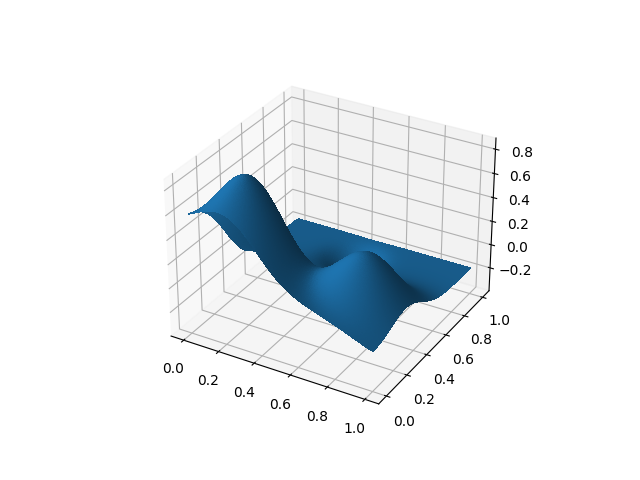
\includegraphics[trim=2.4cm 1cm 1.4cm 1cm, clip,width = 3in]{../assets/actual_franke_plot.png}
  \caption{Shape of Franke's function which will be used as a interpolating goal}
  \label{fig:frankesplot}
\end{figure}

\subsubsection{The Vandermonde matrix applied to Franke's function}


When performing the different regression methods, it is important to sort the data into a well designed system for easy access and easier calculations. The data which is to be used during the calculations is sorted into a so called Vandermonde matrix, which is also known as a design matrix. A Vandermonde matrix is a matrix where the rows is built up by geometric progression \cite{vandermonde}.

Franke's function is a two dimensional function defined by the components $x$ and $y$. Then it is instinctive to have a design matrix $X$ also built up by $x$ and $y$ components into a $n\times p$ matrix, the following way

\begin{equation*}
\mathbf X=  \begin{pmatrix}
   1& x_0 & y_0 & x_0^2 & x_0y_0 & y_0^2 & \ldots & x_0^d y_0^{p-d}\\
    1& x_1 & y_1 & x_1^2 & x_1y_1 & y_1^2 & \ldots & x_1^d y_1^{p-d}\\
    & &  &  &  &  & \vdots & \\
    1 & x_{n-1} & y_{n-1} & x_{n-1}^2 & x_{n-1}y_{n-1} & y_{n-1}^2 & \ldots & x_{n-1}^d y_{n-1}^{p-d}\\
 \end{pmatrix}
\end{equation*}

Where the $d$ is the degree of polynomial. Making the degree higher leads to more complicated equations which naturally gives a more precise regression. Having a design matrix built up by too many terms per polynomial increases the possibility of eventually getting an over fitting model, which will be discussed later in the article.

By having different weights $\beta$ in front of each term in the design matrix, it is possible to calculate how large each term in the polynomials should be in order to make the best approximation. This is the clue of having a design matrix built up by $x$ and $y$ components, making it possible to approximate the polynomials which will fit the Franke's function best. Then the approximation can be written as the following

\begin{equation}
    \hat{\mathbf y}=\mathbf X\beta+\epsilon
\end{equation}

Where $\epsilon$ is the error. This can be written as

\begin{frame}
\footnotesize
\setlength{\arraycolsep}{2.5pt} % default: 5pt
\medmuskip = 1mu % default: 4mu plus 2mu minus 4mu
\begin{equation*}
  \hat{\mathbf y}=  \begin{pmatrix}
    \epsilon_0 & 1 & \beta_0 x_0 &  \beta_1 y_0 &  \beta_2 x_0^2 &  \beta_3 x_0y_0 &  \beta_4 y_0^2 & \ldots &  \beta_5 x_0^d y_0^{p-d}\\
    \epsilon_1 & 1 & \beta_0 x_1 &  \beta_1 y_1 &  \beta_2 x_1^2 &  \beta_3 x_1y_1 &  \beta_4 y_1^2 & \ldots &  \beta_5 x_1^d y_1^{p-d}\\
     & &  &  &  &  & \vdots & \\
    \epsilon_{n-1} & 1 & \beta_0 x_{n-1} & \beta_1 y_{n-1} & \beta_2 x_{n-1}^2 & \beta_3 x_{n-1}y_{n-1} & \beta_4 y_{n-1}^2 & \ldots & \beta_5 x_{n-1}^d y_{n-1}^{p-d}
 \end{pmatrix}.
\end{equation*}
\end{frame}


\begin{comment}
Reference to be added to the bib file:
\end{comment}

\subsection{Linear regression}
The goal of a linear regression model is to find these coefficients $\hat{\mathbf \beta}$, which are best suited for predicting new data via the expression:

\begin{equation*}
  \hat{\mathbf y} = \mathbf X\hat{\mathbf \beta},
\end{equation*}

where $\mathbf X$ is the design matrix constructed from the input data (as explained above), and $\hat{\mathbf y}$ is the resulting prediction. To achieve this, we define a "cost function" of sorts, that evaluates each coefficients ability to predict the initial training dataset. We then find the $\hat{\mathbf \beta}$ that minimizes this cost function. More formally put, we want to find

\begin{equation}
  \hat{\mathbf \beta} = \underset{\beta}{\arg \min}\ C(\beta),
\end{equation}

where $C(\beta)$ is the cost function.


\subsubsection{Ordinary least squares regression ($L_0$)}\label{sec:ols}
Ordinary least squares (OLS) regression uses the residual sum of squares (RSS) function as the cost function. Given $N$ datapoints and the predicted output $\mathbf y$, it reads

\begin{equation}
  \label{eq:rss}
  \text{RSS}(\beta) = \sum_{i=1}^N (y_i - \hat y_i)^2.
\end{equation}

As found in \hyperref[sec:L0_matrix_form]{appendix \ref*{sec:L0_matrix_form}}, a cost function like (\ref{eq:rss}) gives the following matrix equation for $\hat{\mathbf \beta}$

\begin{equation}
  \label{eq:L0_matrix_form}
  \hat \beta = (\mathbf X^T\mathbf X)^{-1}\mathbf X^T \mathbf y
\end{equation}

OLS regression has very low variance, but high bias - as a consequence of the bias-variance tradeoff. This makes OLS regression an "accurate" predictor of its own training data, but susceptible to overfitting, which the following two models are better suited to handle.

\subsubsection{Lasso regression ($L_1$)}
Lasso regression expands upon the above cost function by adding a term that penalizes the size of each coefficient. This is done by a factor of $\lambda$, as shown here:

\begin{equation}
  \label{eq:L1_algo}
  \hat{\mathbf \beta} = \underset{\beta}{\arg \min} \begin{Bmatrix}\sum_{i=1}^N\left(y_i - \beta_0 - \sum_{j=1}^p x_{ij}\beta_j\right)^2 + \lambda \sum_{j=1}^p |\beta_j| \end{Bmatrix} .
\end{equation}

The first sum is from the RSS function, while the second sum is the imposed penalty. The Lasso decreases bias from the OLS model, by decreasing the size of the coefficients, and thus making the variables more equally weighted. 

Lasso regression has no closed form expression for $\hat{\mathbf \beta}$, which means it must be calculated programatically.


\subsubsection{Ridge regression ($L_2$)}\label{rid}
Ridge regression has a penalty corresponding to the coefficient's squared sizes, further decreasing the bias from The Lasso, but obviously also increases variance. It defines $\hat{\mathbf \beta}$ like this

\begin{equation*}
  \hat \beta^{\text{ridge}} = \underset{\beta}{\arg \min} \begin{Bmatrix}\sum_{i=1}^N\left(y_i - \beta_0 - \sum_{j=1}^p x_{ij}\beta_j\right)^2 + \lambda \sum_{j=1}^p \beta_j^2 \end{Bmatrix},
\end{equation*}

which - by the same procedure as shown in \hyperref[sec:L0_matrix_form]{appenix \ref*{sec:L0_matrix_form}}, has this closed form expression

\begin{equation}
  \hat \beta^{\text{ridge}} = (\mathbf X^T\mathbf X + \lambda \mathbf I)^{-1}\mathbf X^T\mathbf y.
\end{equation}

% -----------------------------------
\subsection{Assessment}
\subsubsection{$K$-fold cross-validation}
When faced with the issue of a small dataset, a good solution to circumvent issues during assessment is to utilize whats called $K$-fold cross-validation. It involves splitting the dataset in to $K$ equally sized "folds", and using each fold sequentially as the validation set, whilst training on the others. Say, for example, that we set $K=6$. In this example we would first train our model on the last $5$ datasets and evaluate the skill of our model by trying to predict the first. The evaluation is done by calculating the $R^2$ score, MSE or similar. Thereafter, we use the second fold as the testing set, train on the others, and so forth. The final cross-validation value is the mean of all the calculated statistics.

This is especially a great tool when trying to find the best parameter $\alpha$ present in a model to minimize a certain error/statistic. Cross-validation will then serve as a function we want to minimize to achieve the best result, namely

\begin{equation}
  \text{CV}(\hat f, \alpha) = \frac{1}{N}\sum_{i=1}^N L\left(y_i, \hat f^{-\kappa(i)}(x_i, \alpha)\right)
\end{equation}

where $L$ is the error function we want to optimize, $y_i$ are the true values, $\hat f^{-k}$ is the fitted function excluding the fold $k$ and $\kappa(i)$ is the function taking in the index of the original dataset and returning the fold containing it. 

% -----------------------------------
\subsubsection{The Bootstrap}
Bootstrapping is another validation method that effectively resamples a smaller dataset. It involves creating $B$ bootstraping samples, each the same size of the original dataset. The data points in each sample are drawn from the original dataset randomly with replacement, which means data points can appear multiple times in the same bootstrapping set. For each bootstrapping set, the desired statistic (in our case, the MSE, bias or variance) is calculated and the mean over all bootstrapping sets is the final bootstrap value of said statistic.

\subsection{Bias-variance decomposition}\label{sec:bv_decomp}
Consider a dataset \ensuremath{\mathcal{L}} consisting of the data \ensuremath{\mathbf{X}_\mathcal{L}=\{(y_j, \boldsymbol{x}_j)} for \ensuremath{j=0\ldots n-1\}}. We assume that the true data is generated from the noisy model

\begin{align}
    \mathbf{y}=f(\mathbf{x})+\boldsymbol{\epsilon}, 
    \label{eq:y}
\end{align} where \ensuremath{\boldsymbol{\epsilon}} is the normal distributed noise with zero mean and a standard deviation \ensuremath{\sigma^2}. For the sake of simplicity we consider OLS. In \cref{sec:ols} defined a approximation to the function \ensuremath{f(\mathbf{x})} in terms of the parameters \ensuremath{\boldsymbol{\beta}} and the design matrix \ensuremath{\mathbf{X}} which embody our model, that is \ensuremath{\mathbf{\tilde{y}}=\mathbf{X}\boldsymbol{\beta}}. The parameters \ensuremath{\boldsymbol{\beta}} can then be found by optimizing the mean squared error via the so-called cost function

\begin{align}
    C(\mathbf{X}, \boldsymbol{\beta}) = \frac{1}{n}\sum_{i=0}^{n-1}(y_i-\tilde{y}_i)^2=\mathbb{E}\left[(\mathbf{y}-\mathbf{\tilde{y}})^2\right].
    \label{eq:cost-function}
\end{align} We want to decompose \cref{eq:cost-function} so that it can be expressed as the sum of bias, variance and the standard deviation. This derivation can be found in \hyperref[sec:bv_decomp]{appendix \ref*{sec:bv_decomp}}, where we obtain the result
\begin{align}
    \mathbb{E}\left[(\mathbf{y}-\mathbf{\tilde{y}})^2\right]&=\frac{1}{n}\sum_i(f_i-\mathbb{E}\left[\mathbf{\tilde{y}}\right])^2+\frac{1}{n}\sum_i(\tilde{y}_i-\mathbb{E}\left[\mathbf{\tilde{y}}\right])^2+\sigma^2\\
    &=\mathrm{Bias}[\mathbf{\tilde{y}}]^2+\sigma^2+\mathrm{Var}[\mathbf{\tilde{y}}].
\end{align}
\end{document}
